% Chapter Template

\chapter{Results} % Main chapter title

\label{Chapter6} % Change X to a consecutive number; for referencing this chapter elsewhere, use \ref{ChapterX}

\lhead{Chapter 6. \emph{Results}} % Change X to a consecutive number; this is for the header on each page - perhaps a shortened title

%----------------------------------------------------------------------------------------
%	SECTION 1
%----------------------------------------------------------------------------------------
\section{Error Analysis}
\subsection{Call Options}

\begin{figure}[htbp]
  \centering
    \includesvg[scale=0.38]{Figures/BS_preds_call.svg}
    \rule{35em}{0.5pt}
  \caption[Black-Scholes - Call]{Black-Scholes - Call}
  \label{fig:bs_preds_call}
\end{figure}

\begin{figure}[htbp]
  \centering
    \includesvg[scale=0.38]{Figures/NN_preds_call.svg}
    \rule{35em}{0.5pt}
  \caption[Vanilla Neural Network - Call]{Vanilla Neural Network - Call}
  \label{fig:nn_preds_call}
\end{figure}

In Figure ~\ref{fig:bs_preds_call}, we can see that the difference between the LTP and the predicted value of the option premium by Black-Scholes model is very high. Comparing this with predictions of the Vanilla Neural Network in Figure ~\ref{fig:nn_preds_call}, the predicted values are much closer to LTP.

The value of the mean absolute error for Black-Scholes is 740.16 while that of Vanilla Neural Network is 149.59.

\subsection{Put Options}

Similar to what we have seen in the case of call options, in Figure ~\ref{fig:bs_preds_put}, the difference between the LTP and the predicted value of the option premium by Black-Scholes model is very high. But the predictions of the Vanilla Neural Network in Figure ~\ref{fig:nn_preds_put} are much closer to the LTP. 

The value of the mean absolute error for Black-Scholes is 492.75 while that of Vanilla Neural Network is 112.59.

\begin{figure}[htbp]
  \centering
    \includesvg[scale=0.38]{Figures/BS_preds_put_scaled.svg}
    \rule{35em}{0.5pt}
  \caption[Black-Scholes - Put]{Black-Scholes - Put}
  \label{fig:bs_preds_put}
\end{figure}

\begin{figure}[htbp]
  \centering
    \includesvg[scale=0.38]{Figures/NN_preds_put_scaled.svg}
    \rule{35em}{0.5pt}
  \caption[Vanilla Neural Network - Put]{Vanilla Neural Network - Put}
  \label{fig:nn_preds_put}
\end{figure}

\section{Feature Importance}

We use the python package shap\cite{NIPS2017_7062} to examine the importance of each of the input features.

\begin{figure}[htbp]
  \centering
    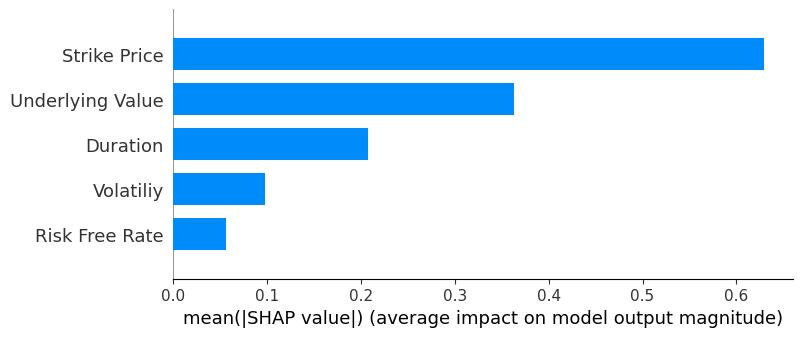
\includegraphics[scale=0.55]{Figures/shap_2.png}
    \rule{35em}{0.5pt}
  \caption[Input Feature Importance - Vanilla Neural Network]{Input Feature Importance - Vanilla Neural Network}
  \label{fig:shap_1}
\end{figure}

Figure ~\ref{fig:shap_1} shows how much important each of the input feature is when calculating option premium. The shap package looks at how much each input feature contributes when calculating the output in the Vanilla Neural Network.
According to the above figure, strike price is the most influential input feature. 

\begin{figure}[htbp]
  \centering
    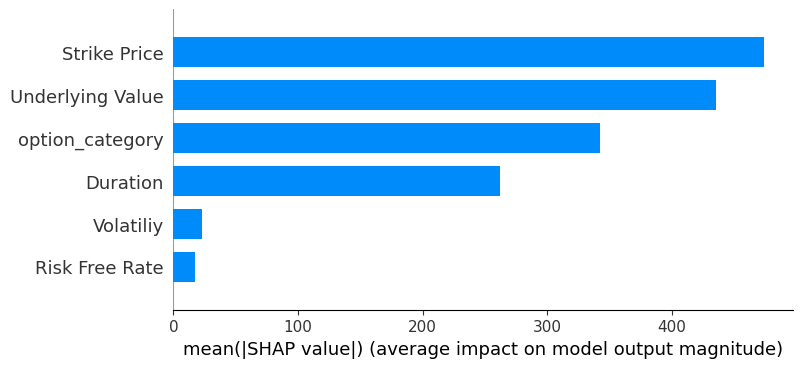
\includegraphics[scale=0.55]{Figures/shap2_combined.png}
    \rule{35em}{0.5pt}
  \caption[Input Feature Importance - Combined Neural Network]{Input Feature Importance - Combined Neural Network}
  \label{fig:shap_1_combined}
\end{figure}

Similarly, for the combined model, we train the model and visualize the importance of the input features. Figure ~\ref{fig:shap_1_combined} shows how the option category is an important feature, which is understandable as even Black-Scholes has different formulas to price put and call options. This graph helps us understand which factors affect the value of an option premium and also helps us rank these factors on a relative scale. This would not be possible with PDE based models like Black-Scholes.  

Apart from showing the significance of each input feature, we can also explore how each of these features is contributing to calculating the output. 

\begin{figure}[htbp]
  \centering
    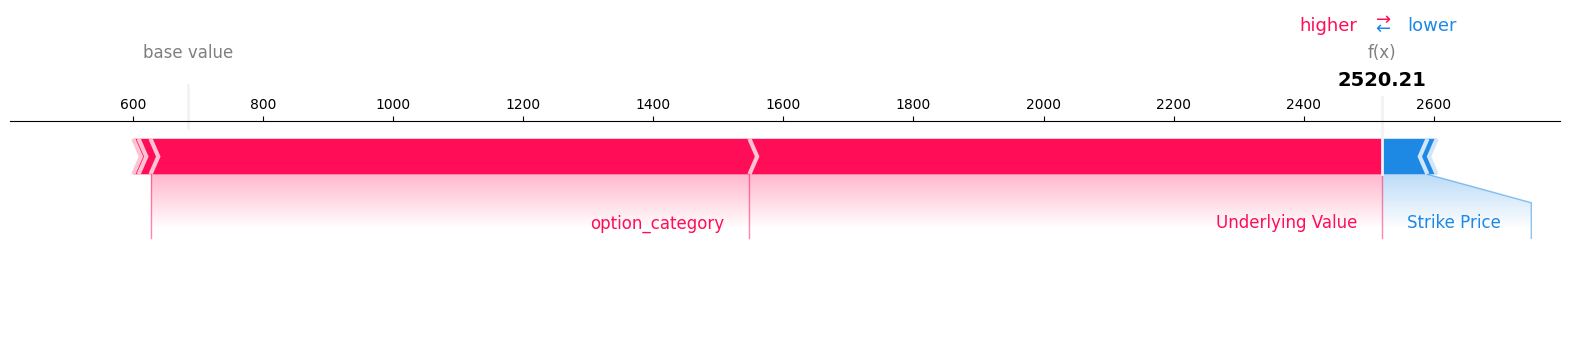
\includegraphics[scale=0.38]{Figures/shap_output_1.png}
    \rule{35em}{0.5pt}
  \caption[Output Calculation - Bar]{Output Calculation - Bar}
  \label{fig:shap_output}
\end{figure}

\begin{figure}[htbp]
  \centering
    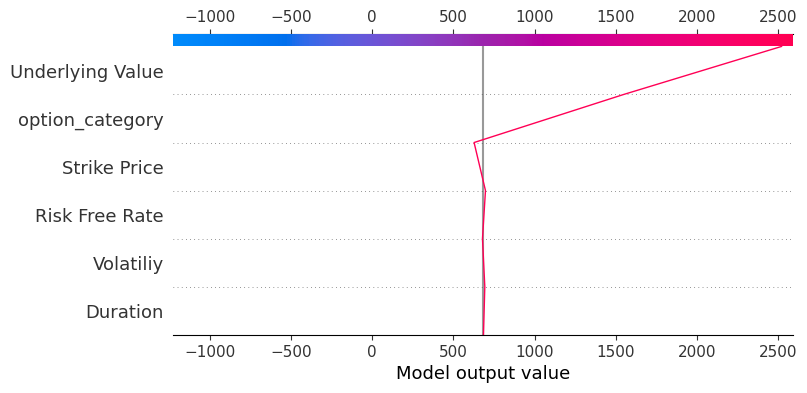
\includegraphics[scale=0.6]{Figures/shap4.png}
    \rule{35em}{0.5pt}
  \caption[Output Calculation - Decision Plot]{Output Calculation - Decision Plot}
  \label{fig:shap_output2}
\end{figure}

Figure ~\ref{fig:shap_output} and ~\ref{fig:shap_output2} show how much each of the input features contribute to this particular model output. It shows both, the magnitude and direction of the impact for all the input features. 

\section{Inference Time}

While these previous sections show how neural networks help improve the accuracy and provide more insight about the important features when predicting option premium, neural networks have one more advantage over PDE based models. 

Comparing the inference time of Black-Scholes and Neural Network based models, it is observed that the Black-Scholes model takes 108 seconds for 409943 data points while Neural Network takes 2.1 seconds for 114045 data points. This shows how the latter is around 14 times faster than traditional PDE based models.   


\section{Conclusion}

Pricing options correctly is important for many reasons. For instance, most of the trading strategies use options as building blocks. Therefore, it is crucial to price them correctly in order to perform the desired strategy correctly. Also, options are used in hedging strategies and hedging is an important aspect of risk mitigation. Overpricing or under pricing of options can lead to huge losses. 

From the results of these various experiments, it is evident that neural networks show a lot of promise in the domain of option pricing. With enough data and compute power, neural networks can learn and understand patterns and relations in the data. All the proposed neural network based models in this work consistently outperform traditional PDE based models by a large margin. Incorporating the option category in the model architecture helps create a unified model to price both the options, which is not possible with Black-Scholes model. Due to the parallelizable nature of neural networks, their inference time is also less as compared to PDE based models. 

% There are some future directions for this work. 

% \begin{figure}[htbp]
%   \centering
% \subfloat[Black-Scholes]{    \includesvg[width=0.6\textwidth]{Figures/BS_preds_call.svg}}
% \subfloat[Vanilla Neural Network]{    \includesvg[width=0.6\textwidth]{Figures/NN_preds_call.svg}}
%     \caption{Model Predictions - Call}
%   \label{fig:data_as_graph}
% \end{figure}

